\documentclass[12pt]{report}
\usepackage[style=ieee]{biblatex}
\addbibresource{references.bib}
\usepackage{enumitem}
\setlist[enumerate]{nosep}
\usepackage{etoolbox}
\usepackage{fancyhdr}
\usepackage{float}
\usepackage{fontspec}
\usepackage[letterpaper,hmargin={47.5mm,17.5mm},top=64.0mm,bottom=25.4mm]{geometry}
\usepackage{indentfirst}
\usepackage{microtype}
\usepackage{multirow}
\usepackage{setspace}
\usepackage{tabularx}
\usepackage[explicit]{titlesec}
\usepackage{tocbibind}
\usepackage{wallpaper}

\newcommand{\authora}{
    Melba Dominique B. Castorico %
}
\newcommand{\authorb}{
    Basil Eric Rabi %
}
\newcommand{\authorc}{
    Herald Joy Dela Cruz %
}
\newcommand{\eg}{\emph{e.g.}}
\newcommand{\hypothesis}[3]{
\noindent \textbf{Research Question:}
\par#1
\begin{quotation}
    \noindent \textbf{Null Hypothesis ($H_o$)}:
    \par#2

    \noindent \textbf{Alternative Hypothesis ($H_a$)}:
    \par#3
\end{quotation}
}


\newcommand{\thetitle}{LOMOPTIM: An Optimization Algorithm for Open Pit Mines with Sub-Optimal Conditions}

\usepackage[hidelinks]{hyperref}
\hypersetup{
    pdfborder  = {0 0 0},
    pdfinfo    = {
        Title    = {\thetitle},
        Subject  = {Mine Economics},
        Author   = {\authora and \authorb and \authorc},
        Keywords = {Optimization, Mining, Mine Economics, Strategic Mine Planning}
    }
}

\addtolength{\headwidth}{15pt}
\doublespacing
\renewcommand{\contentsname}{TABLE OF CONTENTS}
\renewcommand{\headrulewidth}{0pt}
\setmainfont[Mapping=tex-text-ms]{XITS}
%\setmainfont[Mapping=tex-text-ms]{Times New Roman} % TODO: set up Times New Roman in github workflow
\setlength{\headheight}{15pt}
\setlength{\parindent}{12.7mm}
\setcounter{secnumdepth}{3}
\titleformat{\chapter}[block]{\bfseries\centering}{}{0em}{#1}
\titlespacing{\chapter}{0pt}{-30pt}{0pt}
\titlespacing{\section}{0pt}{0pt}{0pt}
\titlespacing{\subsection}{0pt}{0pt}{0pt}
\titlespacing{\subsubsection}{0pt}{0pt}{0pt}

\begin{document}

\ULCornerWallPaper{1}{spus.pdf}
\pagenumbering{roman}
\addcontentsline{toc}{chapter}{TITLE PAGE}
\thispagestyle{empty}

\begin{center}

\textbf{\MakeUppercase{\thetitle}}

\vspace{1.5cm}
A Thesis Proposal Presented to \\
The Faculty of the College of Engineering \\
St. Paul University Surigao \\
Surigao City

\vfill

In Partial Fulfillment \\
of the Requirements for the Degree \\
BACHELOR OF SCIENCE IN MINING ENGINEERING

\vspace{1cm}
By:

\vspace{1cm}
\textbf{\authora} \\

\vspace{1cm}
November 2023

\end{center}

\fancypagestyle{plain}{
    \fancyhead{}
    \fancyfoot{}
    \fancyhead[R]{\thepage}
}

\pagestyle{fancy}
\fancyhead{}
\fancyfoot{}
\fancyhead[R]{\thepage}

\tableofcontents

\titleformat{\chapter}[block]{\bfseries\centering}{CHAPTER \thechapter\\#1}{0em}{}
\titleformat{\section}[block]{\bfseries\centering}{\MakeUppercase{#1}}{0em}{}
\titleformat{\subsection}[block]{\bfseries}{#1}{0em}{}
\titleformat{\subsubsection}[block]{}{\emph{#1}}{0em}{}

\chapter{THE PROBLEM AND ITS BACKGROUND}

\pagenumbering{arabic}

\section{Introduction}

\subsection{Mineral Reserves and Optimized Strategic Plans for Surface Mines}

In surface minining, the maximum area for extraction of ore at any one time shall be dependent on the scall of the mining operation.
For projects that have a processing plant or those with long term supply agreement with domestic processing plant, the maximum disturbed area for extraction shall not exceed to one hundred sixty-two (162) hectares or two (2) meridional block. (DAO 2018-19)
Mine planning software that are utiized in scoping, feasibility, life-of-mine scheduling and in the ongoing re-evaluation of mine plans through production phase.
Accurate evaluation of financial viability of the mineral deposit and development, then determination of the optimal long term strategic mine plan and schedule to extract the full value of that deposit over the life of the mine. 
However, the Algorithm that analysis the conditions for scheduling includes strategic scheduling, detailed cost, price and recovery modelling, multiple scenario analysis, blending, cut-off and simultaneous stockpile optimization and failed to consider the open area for extraction of ore as mandate by existing guidelines. 
Thus, full potential of mine project is not fully attained.
Simultaneous mine production and mine rehabilitation is the major focus on the developement of this algorithm for attainment of the optimum life-of-mine.

\subsubsection{Optimized Economics}
Economic optimization enatails striving to acquire the best from economy in terms of profits, production, and utility.
In entails maximinzing the objective functions which contribute towards the best economic outcome.


\subsubsection{Good Governance and Environmental Compliance}
Environmental resources is essential in economic advancement and the improvement of society's quality of life, and strong environmental governance in important in acheiving goals in sustainable way. 
Mining assumes governance as key to the environment and, as a consequence, to the business.
Simultaneous mining activity and enviromental compliance is one of the sigifi


% Whittle and other alternatives

\subsubsection{Open Area Restriction}


\subsection{Auditability}

\section{Conceptual Framework of the Study}

\section{Statement of the Problem}

\begin{enumerate}
    \item How is the system developed in relation to
            \begin{enumerate}
                \item Software stack selection
                \item Current tools used by the company
                \item End-user's requirement and feedback
            \end{enumerate}
    \item How efficient is the researcher's system terms of
        \begin{enumerate}
            \item Processing time in achieving the highest net present value
            \item Achieving the throughput requirement per product
            \item Achieving the yearly slices which complies to the environmental requirements
        \end{enumerate}
    \item What is the evaluation of the system by the experts and users in terms of
        \begin{enumerate}
            \item Efficiency
            \item User's experience
        \end{enumerate}
\end{enumerate}

\section{hypothesis}

\hypothesis{
Does the researcher's system meet the technical expert's standards in terms of the system's efficiency and user's experience?
}{
The researcher's system did not meet the technical expert's standards based on the identified factors.
}{
The researcher's system meets the technical expert's standards based on the identified factors.
}

\hypothesis{
Are there any technical limitations that might hinder the system's adoption?
}{
There are technical limitations that might hinder the system's adoption.
}{
There are no technical limitations that might hinder the system's adoption.
}

\hypothesis{
Does the researcher's system address the identified challenges and problems?
}{
The researcher's system does not address the identified challenges and problems.
}{
The researcher's system addresses the identified challenges and problems.
}

\section{Significance of the Study}

The objective of the study is to produce a working application which will determine an economically optimum yearly mining sequence from an arbitrary start up to the end of the mine life while prioritizing sub-optimal restrictions like a minimum annual product throughput and a maximum open area at the end of every year.
This study will leverage the programming language C++\cite{cpp} along with the graphical toolkit Qt\cite{qt}.
This study makes it possible to create a repeatable and auditable process in creating life-of-mine plans.

This study is in-line with the goal of good governance of the mining industry through the prioritazation of legal compliance while also taking in consideration the optimum economics.
The proposed system also hosts a feature that exports yearly pit shells in Standford Polygon format \cite{ply} which is viewable in most 3D viewers.

\section{Scope and Limitation of the Study}

The development of the application focuses only on the case of Taganito Mining Coporation (TMC) which has a partner plant using the High Pressure Acid Leach technology.
This plant requires a consistent throughput of limonite ore while TMC's mine product is saprolite ore.
Thus, this study will only account for two products for the mine optimization: limonite and saprolite.

In addition, the programming side of the application will be done in Fedora Linux \cite{fedora} since the programming toolkits such as the C++ compilers, Qt libraries, and data processing tools such as Postgresql \cite{postgres} and PostGIS \cite{postgis} are readily available.

\chapter{REVIEW OF RELATED LITERATURE}

\section{Existing Tools and Algoritms}

\subsection{Lerch-Grossman}

The most common algoritm used in mine optimization is the algoritm described by Helmut Lerch and Ingo Grossman.
This can be illustrated with each mine block with both downward force (cost) and upward force (revenue value).
The objective of this algorithm is to maximize the total upward force without accounting for the mining sequence \cite{IMS}.

\subsection{Pseudoflow}

A variation of the Lerch-Grossman algorithm (LG) which adapted a network analysis of directed graphs and spanning trees is called the pseudoflow.
Although there are also lots of variations of this algoritm, the best variants chosen in most literatures are lowest label and highest label methods \cite{pseudoflow}.

\subsection{GEOVIA Whittle}

GEOVIA Whittle is proprietary strategic mine planning tool which is commonly used in the Phillipines by various surface mines.
This application implements the abovementioned algorithms in mine optimization, Lerch-Grossman and Pseudoflow, while maximizing the Net Present Value of the generated annual pit shells \cite{whittle}.

\subsection{Limitations of GEOVIA Whittle and Its Algorithms}

Although commonly used in the Phillipines, GEOVIA Whittle at present cannot conform to the recent developments of laws related to mining such as the DAO 2018-19 \cite{DAO2018-19} which limits the open area of all mines since GEOVIA Whittle focuses only on addressing engineering design constraints and economic optimization.
In addition, GEOVIA Whittle is able to consider a minimum extraction limit but cannot set a minimum production limit for a specific product.
In the present mineral prices, saprolite ore is more valuable than limonite ore so GEOVIA Whittle will prioritize saprolite ore in the annual production instead of the limonite ore.
However, in the case of Taganito Mine where a minimum production of limonite ore is required to sustain a High Pressure Acid Leach plant, using GEOVIA Whittle will only a produce an unacceptable yearly production.

\section{Development Tools}

\subsection{C++}

The programming language to be used in the development of LOMOPTIM will be C++.
This a high level language which applies object-oriented programming for easier data abstraction.
It also implements easier memory management through the use smart pointers and efficient use of multi-threaded machines through threading and mutual exclusions \cite{cpp}.

\subsection{Qt}

In the creation of the graphical user interface of LOMOPTIM, the C++ toolkit called Qt will be used.
Qt is a graphical toolkit built for C++ which already contains a lot of libraries of graphical elements.
Included in this toolkit is the graphical designer which will allow the reaserchers to design an interface without writing a single line of code \cite{qt}.

\chapter{METHODS}

\section{Research Design}

This study aims to design and develop an application which will mainly comprise of systems designing and writing of software components.
Thus, a multi-phase iterative design as discussed by Leedy and Ormrod will be applied.
This research design is used commonly in design-based research wherein the researchers apply existing knowledge to create more effective systems \cite{MixedMethod}.

\section{Participants}

LOMOPTIM will be tested mostly by the mine planners in Taganito Mine and possibly other mine planners of other operating mines of Nickel Asia Corporation.
The researchers will formulate a method of preparing the sample data input.
The output of LOPTIM will then be compared with in GEOVIA Whittle by the participating mine planners.

\section{Methodology}

\subsection{System Design}

\subsubsection{Use Case}

The basic use case \cite{usecase} of LOMOPTIM is illustrated in Figure~\ref{fig:usecase}.

\begin{figure}[p]
    \centering
    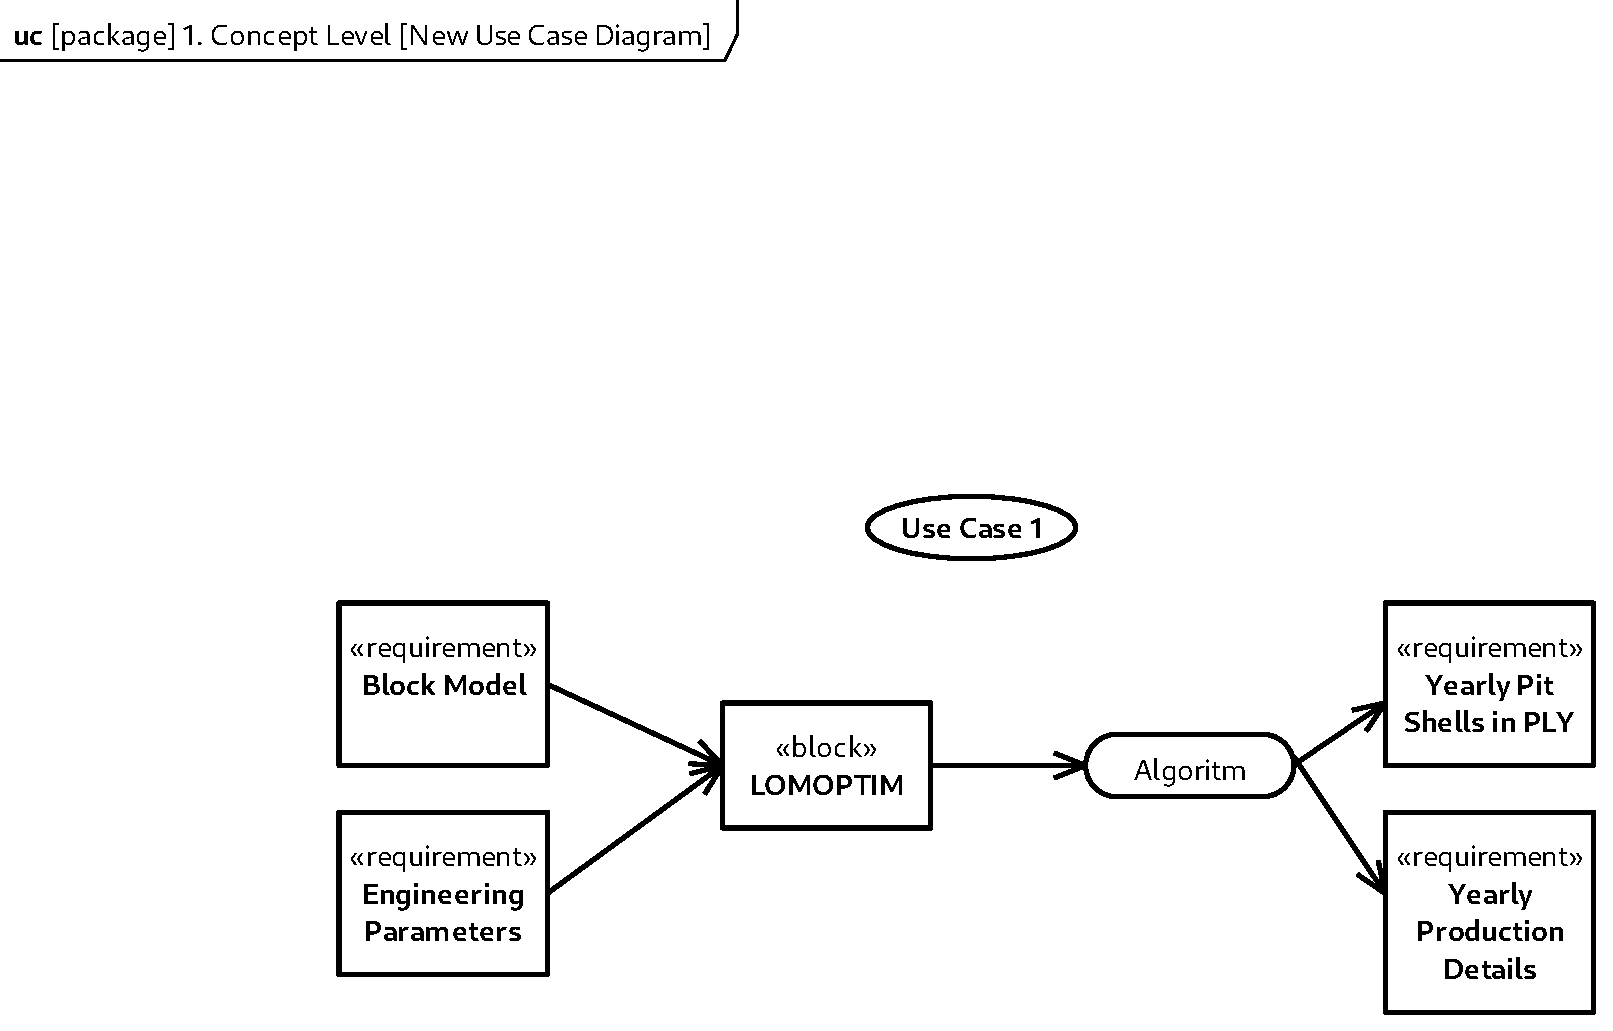
\includegraphics[clip, trim=0 0 0 12mm, width=\linewidth]{img/usecase.pdf}
    \caption{Initial use case of LOMOPTIM.}
    \label{fig:usecase}
\end{figure}

\subsubsection{File Structures}

\subsubsection{Data Structures}

\subsubsection{Algorithm}

\subsection{Source Code Writing}

\subsection{System Testing}

\section{Instruments}

During the development of LOMOPTIM, free and open source tools will be used as discussed in the review of related literature.

In the method of qualitative evaluation, a similar method based on the ER Mine Tracer research design will be applied wherein the researchers of the said study used survey to qualitatively evaluate ER Mine Tracer's functionality and efficiency \cite{ERMineTracer}.

In the preparation of data, data management tools such as PostreSQL \cite{postgres}, PostGIS \cite{postgis}, and R \cite{R} will be used.

\section{Data Gathering Procedure}

\subsection{Quantitative Data}

The efficiency and effectiveness of LOMOPTIM will be evaluated in terms of compliance with the input restrictions and processing time.

\subsection{Qualitative Data}

Qualitative data will be collected through the use of questionnaires to the potential users, engineers, and technology experts if available.
Each question will be have a corresponding point system similar to the Liker 4-point scale \cite{Likert}.

\section{Data Analysis}

The performance of LOMOPTIM will be compared to Whittle which is the existing system used by TMC.
The researchers will be using R version 4.3 \cite{R} to analyze the quantitative data.

Questionnaire surveys with qualitative information will be distributed to Strategic Mine Planners, IT Experts, Computer Engineers and other experts on this topic in order to collect data that are qualitative in nature.

The result of the surveys and the collected quantitative data will be used by the researchers to determine if LOMOPTIM meets the user's requirements, meets the standard's of the technical experts, and does not have any technical limitations that might hinder its adoption.


\titleformat{\chapter}[block]{\bfseries\centering}{}{0em}{#1}
\printbibliography[
    title = {REFERENCES},
    heading = bibintoc
]

\newgeometry{hmargin={47.5mm,20mm},top=64.0mm,bottom=25.4mm}
\setlength{\parindent}{0mm}

\begin{spacing}{1.55}

\chapter*{CURRICULUM VITAE}
\addcontentsline{toc}{chapter}{CURRICULUM VITAE}

\begin{tabularx}{\linewidth}{@{}lXr}
    \MakeUppercase{\authora} && \multirow{3}{*}{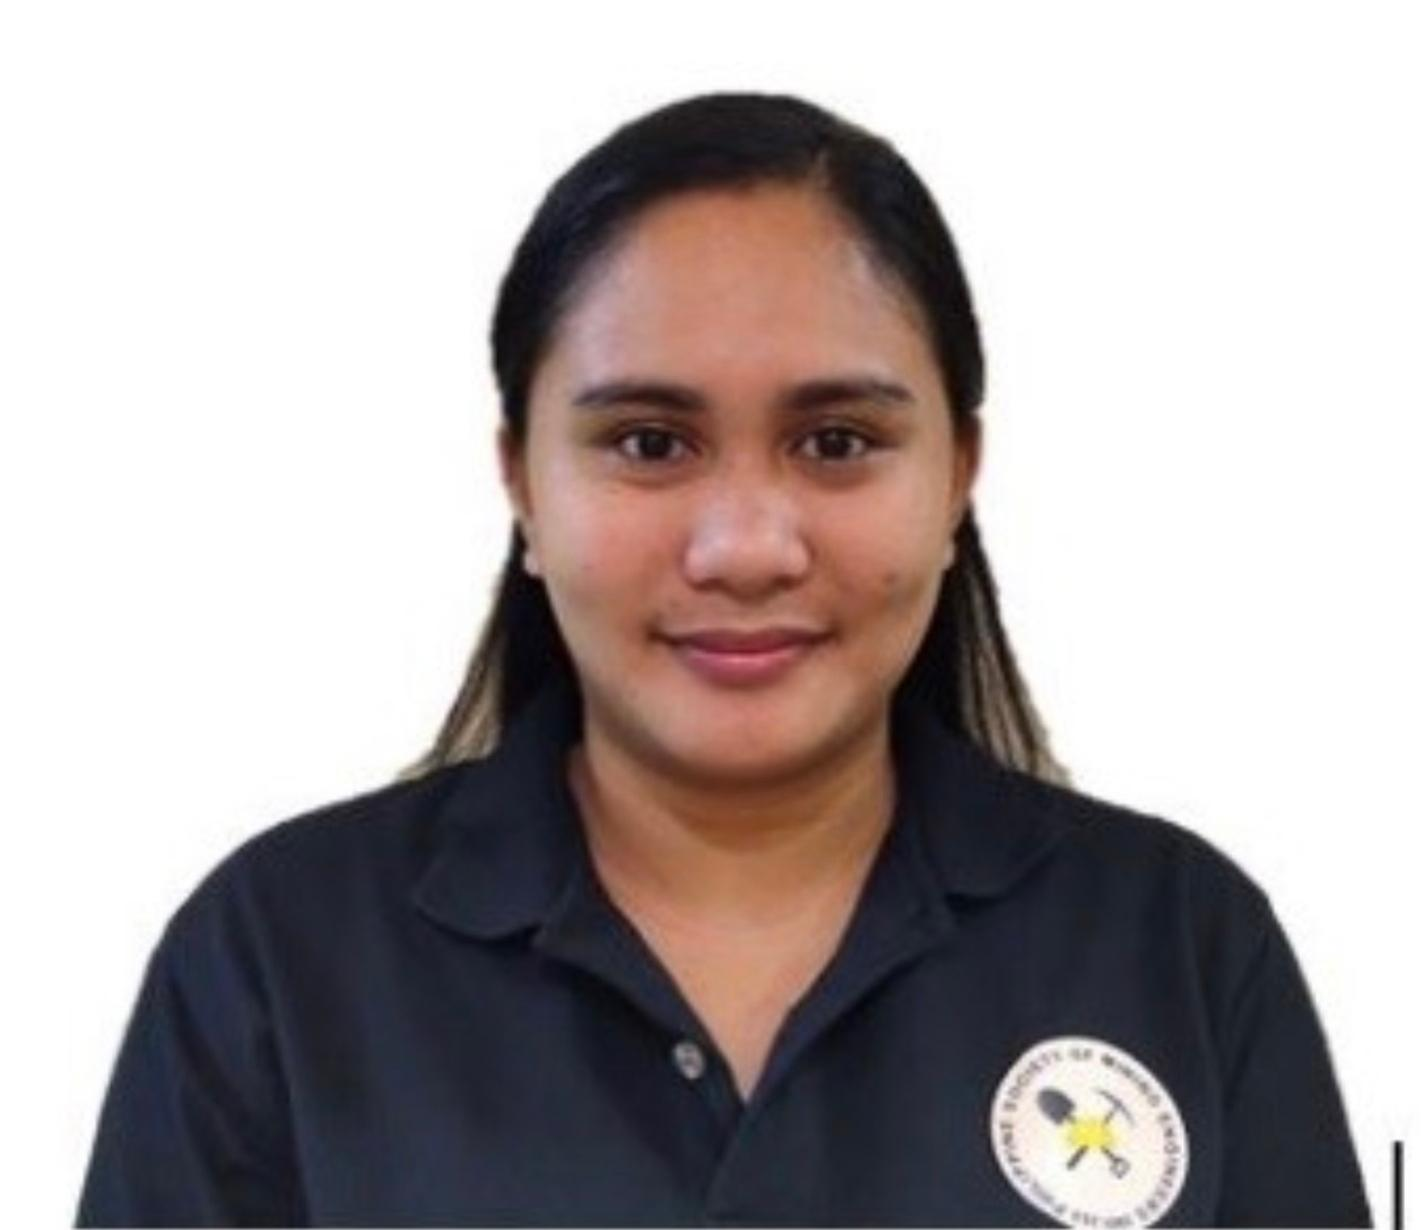
\includegraphics[width=1in]{img/burdeos}} \\ %TODO: Picture
    Bonbon, Butuan City, Agusan del Norte && \\
    melba.dominque@gmail.com && \\
\end{tabularx}

\vspace{20pt}

\textbf{PERSONAL INFORMATION}

\vspace{-10pt}
\hrulefill

\begin{tabular}{@{}l@{ : }l}
    DATE OF BIRTH & June 1, 1992 \\
    PLACE OF BIRTH & Butuan City \\
    AGE & 31 \\
    GENDER & Female \\
    NATIONALITY & Filipino \\
    RELIGION & Catholic \\
    CIVIL STATUS & Married \\
    FATHER'S NAME & Michael B. Burdeos \\
    MOTHER'S NAME & Josephine A. Burdeos \\
\end{tabular}

\vspace{20pt}

\textbf{EDUCATIONAL BACKGROUND}

\vspace{-10pt}
\hrulefill

\begin{tabular}{@{}l@{ : }l}
    COLLEGE & Saint Paul University Surigao \\
    & Corner Rizal and San Nicolas Streets, Surigao City \\
    HIGH SCHOOL & Agusan National High School\\
    & A.D. Curato St., Butuan City \\
    ELEMENTARY & La Trinidad Elementary School \\
    & Bonbon, Butuan City \\
\end{tabular}

\end{spacing}
\end{document}
